%-------------------------------------------------------------------------------
%	PACKAGES AND OTHER DOCUMENT CONFIGURATIONS
%-------------------------------------------------------------------------------

\documentclass{article}

% Packages
% Packages

% \usepackage{fancyhdr} % Required for custom headers
% \usepackage{lastpage} % Required to determine the last page for the footer
% \usepackage{extramarks} % Required for headers and footers
% \usepackage[usenames,dvipsnames]{color} % Required for custom colors
\usepackage{graphicx} % Required to insert images
% \usepackage{listings} % Required for insertion of code
% \usepackage{courier} % Required for the courier font
% \usepackage{dsfont} % For special math characters
% \usepackage{verbatim}

%\usepackage{amsmath, amssymb, bm} % For matrix notation
\usepackage[english]{babel}
\usepackage[paperwidth=8.5in,paperheight=11in,margin=1.0in]{geometry}
\usepackage{listings}
\usepackage{hyperref}
%\usepackage[cmex10]{amsmath, bm}
\usepackage{amsmath, bm}
\usepackage{blkarray}








% formatting
\pdfcompresslevel0

% ==============================================================================
% PYTHON
% ==============================================================================
\usepackage[utf8]{inputenc}

% Default fixed font does not support bold face
\DeclareFixedFont{\ttb}{T1}{txtt}{bx}{n}{12} % for bold
\DeclareFixedFont{\ttm}{T1}{txtt}{m}{n}{12}  % for normal

% Custom colors
\usepackage{color}
\definecolor{deepblue}{rgb}{0,0,0.5}
\definecolor{deepred}{rgb}{0.6,0,0}
\definecolor{deepgreen}{rgb}{0,0.5,0}

\usepackage{listings}

% Python style for highlighting
\newcommand\pythonstyle{\lstset{
language=Python,
basicstyle=\ttm,
otherkeywords={self},             % Add keywords here
keywordstyle=\ttb\color{deepblue},
emph={MyClass,__init__},          % Custom highlighting
emphstyle=\ttb\color{deepred},    % Custom highlighting style
stringstyle=\color{deepgreen},
frame=tb,                         % Any extra options here
showstringspaces=false,            % 
breaklines=true
}}


% Python environment
\lstnewenvironment{python}[1][]
{\pythonstyle\lstset{#1}
}
{}

% Python for external files
\newcommand\pythonexternal[2][]{{
\pythonstyle\lstinputlisting[#1]{#2}}}

% Python for inline
\newcommand\pythoninline[1]{{\pythonstyle\lstinline!#1!}}
% ==============================================================================
% ==============================================================================

% Margins
\topmargin=-0.45in
\evensidemargin=0in
\oddsidemargin=0in
\textwidth=6.5in
\textheight=9.0in
\headsep=0.25in

\linespread{1.1} % Line spacing

% Set up the header and footer
\pagestyle{fancy}
\lhead{\hmwkAuthorName} % Top left header
\chead{\hmwkClass\ (\hmwkClassInstructor\ \hmwkClassTime): \hmwkTitle} % Top center head
\rhead{\firstxmark} % Top right header
\lfoot{\lastxmark} % Bottom left footer
\cfoot{} % Bottom center footer
\rfoot{Page\ \thepage\ of\ \protect\pageref{LastPage}} % Bottom right footer
\renewcommand\headrulewidth{0.4pt} % Size of the header rule
\renewcommand\footrulewidth{0.4pt} % Size of the footer rule

\setlength\parindent{0pt} % Removes all indentation from paragraphs

%----------------------------------------------------------------------------------------
%	DOCUMENT STRUCTURE COMMANDS
%	Skip this unless you know what you're doing
%----------------------------------------------------------------------------------------

% Header and footer for when a page split occurs within a problem environment
\newcommand{\enterProblemHeader}[1]{\nobreak\extramarks{#1}{#1 continued on next page\ldots}\nobreak\nobreak\extramarks{#1 (continued)}{#1 continued on next page\ldots}\nobreak}

% Header and footer for when a page split occurs between problem environments
\newcommand{\exitProblemHeader}[1]{\nobreak\extramarks{#1 (continued)}{#1 continued on next page\ldots}\nobreak\nobreak\extramarks{#1}{}\nobreak}

\setcounter{secnumdepth}{0} % Removes default section numbers
\newcounter{homeworkProblemCounter} % Creates a counter to keep track of the number of problems

\newcommand{\homeworkProblemName}{}
\newenvironment{homeworkProblem}[1][Problem \arabic{homeworkProblemCounter}]{ % Makes a new environment called homeworkProblem which takes 1 argument (custom name) but the default is "Problem #"
\stepcounter{homeworkProblemCounter} % Increase counter for number of problems
\renewcommand{\homeworkProblemName}{#1} % Assign \homeworkProblemName the name of the problem
\section{\homeworkProblemName} % Make a section in the document with the custom problem count
\enterProblemHeader{\homeworkProblemName} % Header and footer within the environment
}{\exitProblemHeader{\homeworkProblemName} % Header and footer after the environment
}

% Defines the problem answer command with the content as the only argument
\newcommand{\problemAnswer}[1]{\noindent\framebox[\columnwidth, resolution=600][c]{\begin{minipage}{0.98\columnwidth, resolution=600}#1\end{minipage}}}
% Makes the box around the problem answer and puts the content inside }

\newcommand{\homeworkSectionName}{}
\newenvironment{homeworkSection}[1]{ % New environment for sections within homework problems, takes 1 argument - the name of the section
\renewcommand{\homeworkSectionName}{#1} % Assign \homeworkSectionName to the name of the section from the environment argument
\subsection{\homeworkSectionName} % Make a subsection with the custom name of the subsection
\enterProblemHeader{\homeworkProblemName\ [\homeworkSectionName]} % Header and footer within the environment
}{
\enterProblemHeader{\homeworkProblemName} % Header and footer after the environment
}



%-------------------------------------------------------------------------------
%	NAME AND CLASS SECTION
%-------------------------------------------------------------------------------

\newcommand{\hmwkTitle}{Homework 8} % Assignment title
\newcommand{\hmwkDueDate}{Friday, Nov 14} % Due date
\newcommand{\hmwkClass}{ECE 532} % Course/class
\newcommand{\hmwkClassTime}{11:00 am} % Class/lecture time
\newcommand{\hmwkClassInstructor}{Robert Nowak} % Teacher/lecturer
\newcommand{\hmwkAuthorName}{Elijah Bernstein-Cooper} % Your name

%-------------------------------------------------------------------------------
%	TITLE PAGE
%-------------------------------------------------------------------------------

\title{\vspace{0in}
    \textmd{\textbf{\hmwkClass:\ \hmwkTitle}}\\
    \normalsize\vspace{0.1in}\small{Due\ on\ \hmwkDueDate}\\
    \vspace{0.1in}\large{\textit{\hmwkClassInstructor\ \hmwkClassTime}}
    \vspace{0.5in}}

\author{\textbf{Elijah Bernstein-Cooper}}
\date{\today} % Insert date here if you want it to appear below your name

%-------------------------------------------------------------------------------

\begin{document}

\maketitle
%\newpage

%===============================================================================
%-------------------------------------------------------------------------------
%	PROBLEM 1
%-------------------------------------------------------------------------------
\begin{homeworkProblem}
   
    We performed a brute force estimate of the dual optimization parameter
    $\alpha$ for hinge loss to classify the four people as basketball players
    or not basketball players. We optimized the following

    \begin{equation}
        {\rm min_{\alpha}} \sum_{i=1}^m \left(1 - b_i\sum_{j=1}^m\alpha_j 
        \bm{a_i}^T \bm{a}_j \right) + \lambda \sum_{i=1}^m \sum_{j=1}^m \alpha_i
        \alpha_j \bm{a}_i^T \bm{a}_j
    \end{equation}

    \noindent where $\alpha$ will be a 4$\times$1 vector of weights, or rather
    the support vector. We derived
  
    \begin{equation}
    \bm{a} = \left(\begin{matrix} -0.8 \\ -0.1 \\ 0 \\ 0.8 \\ 
    \end{matrix} \right)
    \end{equation}

    We wish to derive a best estimate for the weight vector $\bm{x}$ where
    $\bm{b} = \bm{Ax}$, with $\bm{b}$ being a binary vector, 1 for basketball
    player, -1 for not a basketball player, and $\bm{A}$ will be the heights of
    the people. In the dual hinge loss scenario

    \begin{equation}
        \bm{\hat{x}} = \sum_{j=1}^m \alpha_j \bm{a}_j
    \end{equation}

    Our hinge loss optimization produced an optimal classification rule of
    $\bm{\hat{x}} = 0.21$. Using least squares we find an $\bm{\hat{x}}$ of
    0.0076. The least squares classification predicts that all people will be
    basketball players, while the dual hinge loss SVM classification predicts
    the two tallest will be basketball players. See the code at the end of the
    homework.

\end{homeworkProblem}
\clearpage
%===============================================================================

%===============================================================================
%-------------------------------------------------------------------------------
%	PROBLEM 2 
%-------------------------------------------------------------------------------
\begin{homeworkProblem}
  
    We found that the 3rd value of $\bm{\alpha}$ is zero. The support vectors
    are the 1st, 2nd, and 4th values of $\alpha$. We used the dual solution in
    Problem 1, see the same code at the end of the homework.

\end{homeworkProblem}
%===============================================================================

%===============================================================================
%-------------------------------------------------------------------------------
%	PROBLEM 3
%-------------------------------------------------------------------------------
\begin{homeworkProblem}

    We find that changing $t_0 = 0$ changes the classification $\bm{\hat{x}} =
    0$, but we still classify the people 100\% correctly. This likely means
    that the classification is robust to the particular hinge loss chosen.

\end{homeworkProblem}
%===============================================================================

%===============================================================================
%-------------------------------------------------------------------------------
%	PROBLEM 4
%-------------------------------------------------------------------------------
\begin{homeworkProblem}

    We performed a simulation of generating datasets of sizes 10$\times$10,
    100$\times$100, 1000$\times$1000. For each dataset size, we ran 100
    iterations of regenerating the data, and classified the generated data with
    the least squares, Gaussian kernel SVMs, and polynomial kernel SVMs. We
    calculated the percent total of mistakes made by each of the three methods,
    see Table~\ref{table:prob4} for the results. See Figure~\ref{fig:prob4} for
    an example of classifications for a 1000$\times$1000 dataset. See the code
    at the end of the homework.

    \begin{table}[!ht]

        \caption{\label{table:prob4} Resulting \% total classification mistakes
        for different methods and dataset sizes.}

        \begin{center}
            \begin{tabular}{lccc}
                
                & 10$\times$10 & 100$\times$100 & 1000$\times$1000 \\
                \hline \hline
                Least Squares     & 33 & 45 & 48.4 \\
                Gaussian Kernel   & 2  & 2 & 1.3 \\
                Polynomial Kernel & 8  & 3 & 3.9 \\

            \end{tabular}
        \end{center}
    \end{table}
    \begin{figure}[!ht]
        
        \begin{centering}
        
        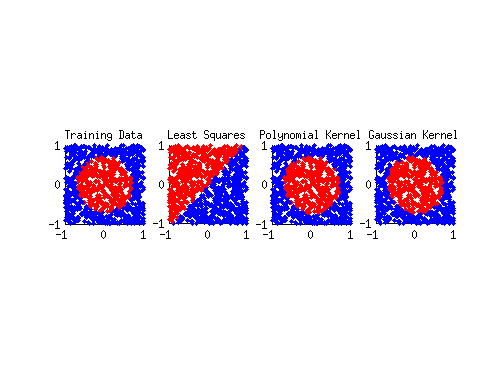
\includegraphics[width=\linewidth]{fig_prob4.png}

        \caption{\label{fig:prob4} Results from classifications of the training
    data. The Gaussian kernel outperforms the least squares and polynomial
    kernel classification.} \end{centering}

    \end{figure} 

\end{homeworkProblem}
%===============================================================================

\clearpage
{\huge Code:}

{\large \bf Problem 1 \& 2} \\
\lstinputlisting{hw8_prob1.m} 
\hrule \hrule

{\large \bf Problem 3} \\
\lstinputlisting{hw8_prob3.m} 
\hrule \hrule

{\large \bf Problem 4} \\
\lstinputlisting{hw8_prob4.m} 
\hrule \hrule

\end{document}

